\documentclass[a4paper, spanish]{exam}
\usepackage[utf8]{inputenc}
\usepackage[spanish]{babel}
\selectlanguage{spanish}
\usepackage[margin=1in]{geometry}
\usepackage{amsmath,amssymb}
\usepackage{multicol}
\usepackage{natbib}
\usepackage{graphicx}

%los de aca abajo capaz no los uso
\newcommand{\class}{Matemática: Evaluación de  Logaritmos}
\newcommand{\term}{2° Trimestre 2015}
\newcommand{\examnum}{Tema 1}
\newcommand{\examprof}{Alexis Gomel}
\newcommand{\examdate}{15/7/2015}
\newcommand{\timelimit}{60 Minutes}%no lo uso


%el header de las hojas.
\pagestyle{head}
\firstpageheader{}{}{}
\runningheader{\class}{\examnum\ - Page \thepage\ of \numpages}{\examdate}
\runningheadrule

\begin{document}
\noindent
\begin{tabular*}{\textwidth}{l @{\extracolsep{\fill}} r @{\extracolsep{6pt}} l}
\textbf{\class} & \textbf{Profesor: \examprof}\\
\textbf{\examnum} & \textbf{\examdate} \\
%\textbf{Time Limit: \timelimit} & Teaching Assistant & \makebox[2in]{\hrulefill}
\textbf{Nombre: } \makebox[2in]{\hrulefill}
\end{tabular*}\\
\rule[2ex]{\textwidth}{2pt}

%%%%%%%%%%%%%%%%%%%%%%%%%%%%%%%%%%%%%%%%%%%




Justificar cada respuesta. El examen esta pensado para que no haga falta usar una calculadora.
\begin{table}[h]
\centering
%\caption{My caption}
\label{my-label}
\begin{tabular}{|l|c|c|c|c|}
\hline
Ejercicio        & 1 & 2 & 3 & Nota \\ \hline
Puntaje maximo   & 4 & 2 & 4 &   10   \\ \hline
Puntaje obtenido &   &   &   &      \\ \hline
\end{tabular}
\end{table}

Si se traban con algún ejercicio, pasen al siguiente y vuelvan a intentar mas tarde con el que dejaron.

\begin{enumerate}
\item (4 Puntos)\textbf{Resolver:} Cada ítem vale medio $0,5$ puntos.
\begin{multicols}{2}
\begin{enumerate}
\item $log(1000)-\frac{1}{3}.log_{1/2}(1)$
\item $4^{log_2(5)}$
\item $log_2(\frac{1}{64})$
\item $e^{3.ln(3) + 2.ln(5) - 2^{6}.ln(1)}$

\columnbreak

\item $log(4+\sqrt{6})+log(4-\sqrt{6})$

Sabiendo que $log_3(5) \simeq 1,46$, calcular:

\item $log_3(15)$
\item $log_5(3)$
\item $log_3(25)$


\end{enumerate}
\end{multicols}

\item (2 Puntos)\textbf{Gráficos:}
Cada ítem vale 1 punto.
\begin{enumerate}
\item Graficar $log_2(2.(x-3))$. (Basta con usar solo 4 puntos)

\item Encontrar $a$ y $b$ ,  a partir del gráfico de $y=log_a(x-b)$

\begin{figure}[h!]
\centering
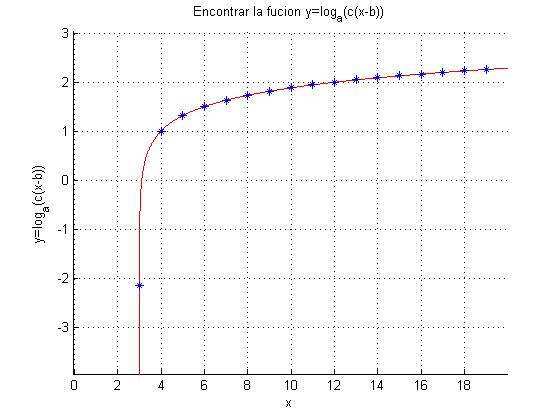
\includegraphics[width=0.6\textwidth]{logsencontrar1.jpg}
\caption{Encontrar $a$,$b$ y $c$,  a partir del gráfico de $y=log_a(x-b)$.
Los asteriscos azules marcan los valores de $y$ para $3,4,5,6,7...$}
\label{fig:logaritmo}
\end{figure}

\end{enumerate}

\item (4 Puntos)\textbf{Encontrar, si es posible, el valor de x :}
Cada item vale 1 punto.
\begin{enumerate}
\item $5^x+2.5^x+5^{x+2}=900$
\item $4.log_3(x)-2.log_9(x)=3 $
\item $log_5(4.x-3)=1$
\item $log(x)=-2.log(m)+4.log(n)-2$
\end{enumerate}
  
 
 
 
\end{enumerate}
\rule[2ex]{\textwidth}{2pt}
 
“There’s as many atoms in a single molecule of your DNA as there are stars in the typical galaxy. We are, each of us, a little universe.”
― Neil deGrasse Tyson, Cosmos 

\newpage

\section*{Respuestas}
1: 1)3 ;2) 25 ;3) -6 ;4)$ 34 (9+25)$ ;5)$ 1+1,46 $ ;6)$ 1/1,46=0,685$ ;7)$2*1,46$ ;8)1

2: ver grafico

3:$log_9(9.(x-3))$

4: 1)2  ;2)1 ;3)2 ;4)$\frac{m^2.n^4}{100}$

\end{document}
